\section{System architecture}
\label{sec:arch}

The application is an Electron~\cite{electron} shell around a TypeScript renderer. The shell
owns windows, the native menu, file dialogues and printing; the renderer owns everything
else. The renderer is bundled by Vite~\cite{vite} into a single script of 660.2\,kB
(197.8\,kB gzip) plus 26.1\,kB of CSS (6.0\,kB gzip). User-interface resources ---
icons and strings that are not code --- are packed into a 19\,kB container with a format of
the project's own, described in the repository.

\begin{figure}[t]
\centering
% Explicit coordinates and a fixed text width: relative placement let a satellite box
% drift over its neighbour, and a figure that is wrong is worse than one that is plain.
\tikzset{
  box/.style={draw=ink!55, rounded corners=2pt, fill=white, align=center,
              font=\small, inner sep=3.2pt, text width=3.5cm, minimum height=8mm},
  side/.style={box, font=\footnotesize, text width=2.7cm, minimum height=7.4mm},
  group/.style={draw=grey!55, dashed, rounded corners=4pt, inner sep=6pt, fill=none},
  lbl/.style={font=\scriptsize\itshape, color=grey},
  ar/.style={-{Latex[length=1.6mm]}, draw=ink!65, thick},
  dep/.style={-{Latex[length=1.6mm]}, draw=ink!45, densely dashed},
}
\begin{tikzpicture}

% left column: the desktop shell
\node[box] (shell) at (0,0) {Electron main process\\\scriptsize windows, menu, dialogues, printing};
\node[box] (bridge) at (0,-1.35) {preload bridge\\\scriptsize typed, explicit surface};

% right column: the renderer
\node[box] (boot) at (7.0,0) {bootstrap\\\scriptsize \texttt{main.ts}, 91 commands};
\node[box] (viewer) at (7.0,-1.35) {viewer\\\scriptsize page list, virtualisation, zoom};
\node[box] (layer) at (7.0,-2.7) {annotation layer\\\scriptsize geometry, gestures, hit test};
\node[box] (model) at (7.0,-4.05) {annotation model\\\scriptsize kinds, store, history};
\node[box] (pdf) at (7.0,-5.4) {PDF layer\\\scriptsize parse $\cdot$ write $\cdot$ rewrite $\cdot$ merge};
\node[box] (engine) at (7.0,-6.75) {pdf.js\\\scriptsize rasterise, text runs};

% satellites, to the right of the column, well clear of it
\node[side] (tools) at (10.55,-2.7) {tools\\\scriptsize find, measure};
\node[side] (ui) at (10.55,-4.05) {UI\\\scriptsize dialogs, sidebar, i18n};

\begin{scope}[on background layer]
  \node[group, fit=(shell)(bridge), label={[lbl]above:desktop shell}] {};
  \node[group, fit=(boot)(viewer)(layer)(model)(pdf)(engine)(tools)(ui),
        label={[lbl]above:renderer (TypeScript, bundled)}] {};
\end{scope}

\draw[ar] (boot) -- (viewer);
\draw[dep] (layer) -- (model);
\draw[dep] (model) -- (pdf);
\draw[dep] (pdf) -- (engine);
\draw[dep] (tools.west) -- (layer.east);
\draw[dep] (ui.west) -- (model.east);
\draw[ar] (bridge.east) -- node[lbl, above]{\scriptsize IPC} (boot.west);
\end{tikzpicture}
\caption{Module layout. The PDF layer is the only component that touches bytes, and it is
independent of the renderer: it parses into its own value types rather than using pdf.js's
object model, which is what allows the writers to copy objects the renderer never looks at.
Solid arrows are calls; dashed arrows are use.}
\label{fig:arch}
\end{figure}

Figure~\ref{fig:arch} shows the layout and Table~\ref{tab:modules} its size. Two decisions
shape everything else.

\paragraph{The PDF layer has its own object model.} pdf.js exposes a document proxy that can
resolve objects, but it does not expose byte offsets, object generations, or the raw text of
an uncompressed object. All three are needed to write an incremental update: the offset is
what a cross-reference entry holds, the generation is part of a reference, and copying an
uncompressed object's bytes verbatim is both faster and safer than re-serialising a parse of
it. The project therefore has its own lexer and parser (\texttt{src/pdf}, eight files), and
uses pdf.js strictly as a rasteriser and text extractor. The duplication is real --- two
parsers over the same bytes --- and is the largest structural cost in the system; it buys
independence from a renderer's internal model, which is the property the writers need.

\paragraph{A page-space coordinate system of our own.} The renderer, the annotation model and
the hit test all work in \emph{unrotated page space at scale 1, origin top-left, $y$ down}.
PDF user space has its origin at the bottom-left and is scaled by the page's
\texttt{UserUnit}, so every conversion is explicit
($y_{\text{pdf}} = \texttt{MediaBox}_3 - y$) and every annotation stores coordinates that
survive a zoom, a rotation or a change of view mode without being rewritten. This sounds
pedantic and is not: the first implementation mixed rotated and unrotated coordinates and
placed marks correctly at 100\,\% and nowhere else.

\begin{figure}[t]
  \centering
  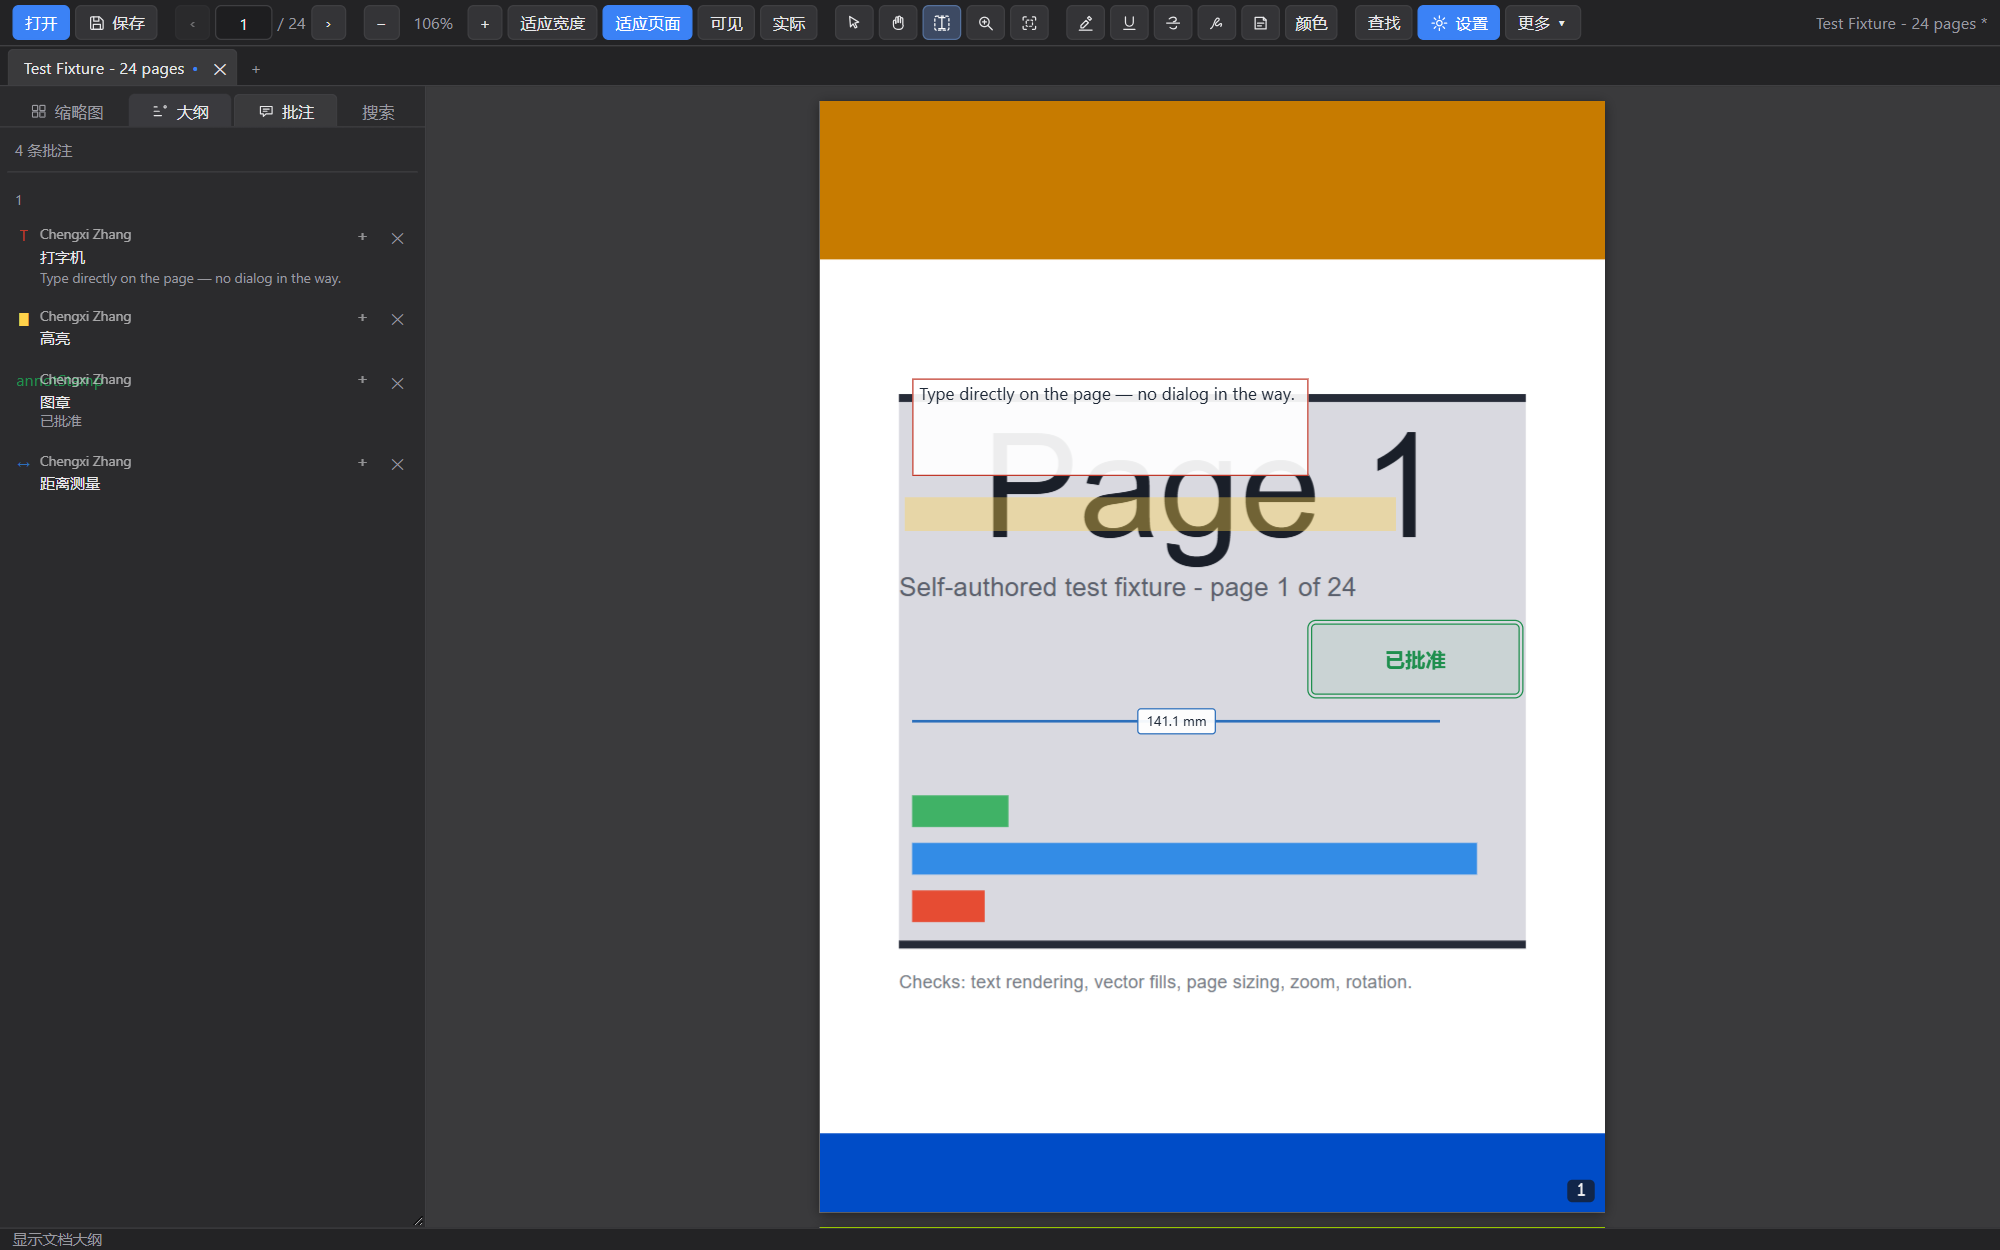
\includegraphics[width=\textwidth]{figures/screenshot.png}
  \caption{The application. The page carries a typewriter box, a text highlight, a standard
  stamp and a distance measurement; the sidebar lists them by kind, page and author. The
  panel matters as much as the page: an annotation that cannot be found again is not much of
  an annotation.}
  \label{fig:screenshot}
\end{figure}

\begin{table}[t]
  \centering
  \caption{Source size. Lines are physical lines of \texttt{.ts}, \texttt{.mjs},
  \texttt{.cjs} and \texttt{.css}; blank lines and comments are included, so the figures
  overstate logical code by roughly a fifth. Measured over the 47 application files and the
  52 test and tooling files.}
  \label{tab:modules}
  \small
  \begin{tabular}{@{}lrr@{}}
    \toprule
    Component & Files & Lines \\
    \midrule
    PDF reader and writers (\texttt{src/pdf}) & 8 & 3{,}349 \\
    Annotations (\texttt{src/annotations}) & 5 & 2{,}146 \\
    Viewer (\texttt{src/viewer}) & 5 & 1{,}334 \\
    UI, dialogs (\texttt{src/ui}) & 5 & 1{,}232 \\
    Tools: find, measure, snapshot (\texttt{src/tools}) & 5 & 972 \\
    i18n and command table (\texttt{src/i18n}) & 7 & 1{,}382 \\
    Sidebar panels (\texttt{src/sidebar}) & 4 & 738 \\
    Tabs and sessions (\texttt{src/tabs}) & 2 & 178 \\
    Saved searches (\texttt{src/search}) & 1 & 91 \\
    Styles & 1 & 1{,}414 \\
    Bootstrap (\texttt{main.ts}, \texttt{product.ts}) & 2 & 3{,}887 \\
    Electron host (\texttt{main.cjs}, \texttt{preload.cjs}) & 2 & 600 \\
    \midrule
    \textbf{Application} & \textbf{47} & \textbf{17{,}323} \\
    Tests and tooling (\texttt{tools/}) & 52 & 10{,}594 \\
    \bottomrule
  \end{tabular}
\end{table}

The 1{,}414 lines of CSS deserve a note: the application has four themes (light, dark, sepia,
high contrast) driven by custom properties on a \texttt{data-theme} attribute, which is why
the stylesheet is larger than several TypeScript modules. The 3{,}887-line bootstrap is the
concentration of failure in this architecture --- 91 commands, their bindings, the menu
descriptor, the debug hooks and the wiring of every module. It is also the file most likely to
be touched by a change, and the one where an omission is silent: a command registered without a
control appears in no menu and reports nothing.
